\section{Appendix 1: Sloan actuators structure}

\begin{figure}[h]
\begin{center}
	\begin{subfigure}{0.22\textwidth}
	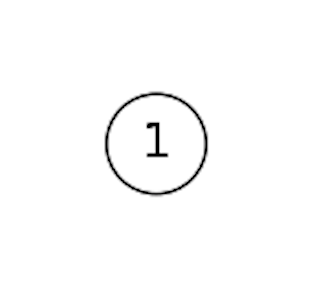
\includegraphics[width=\textwidth]{circles/initialisation}
	\caption{Initialisation.}
	\label{fig:appendix:sloan_structure:initialization}
	\end{subfigure}
	\begin{subfigure}{0.54\textwidth}
	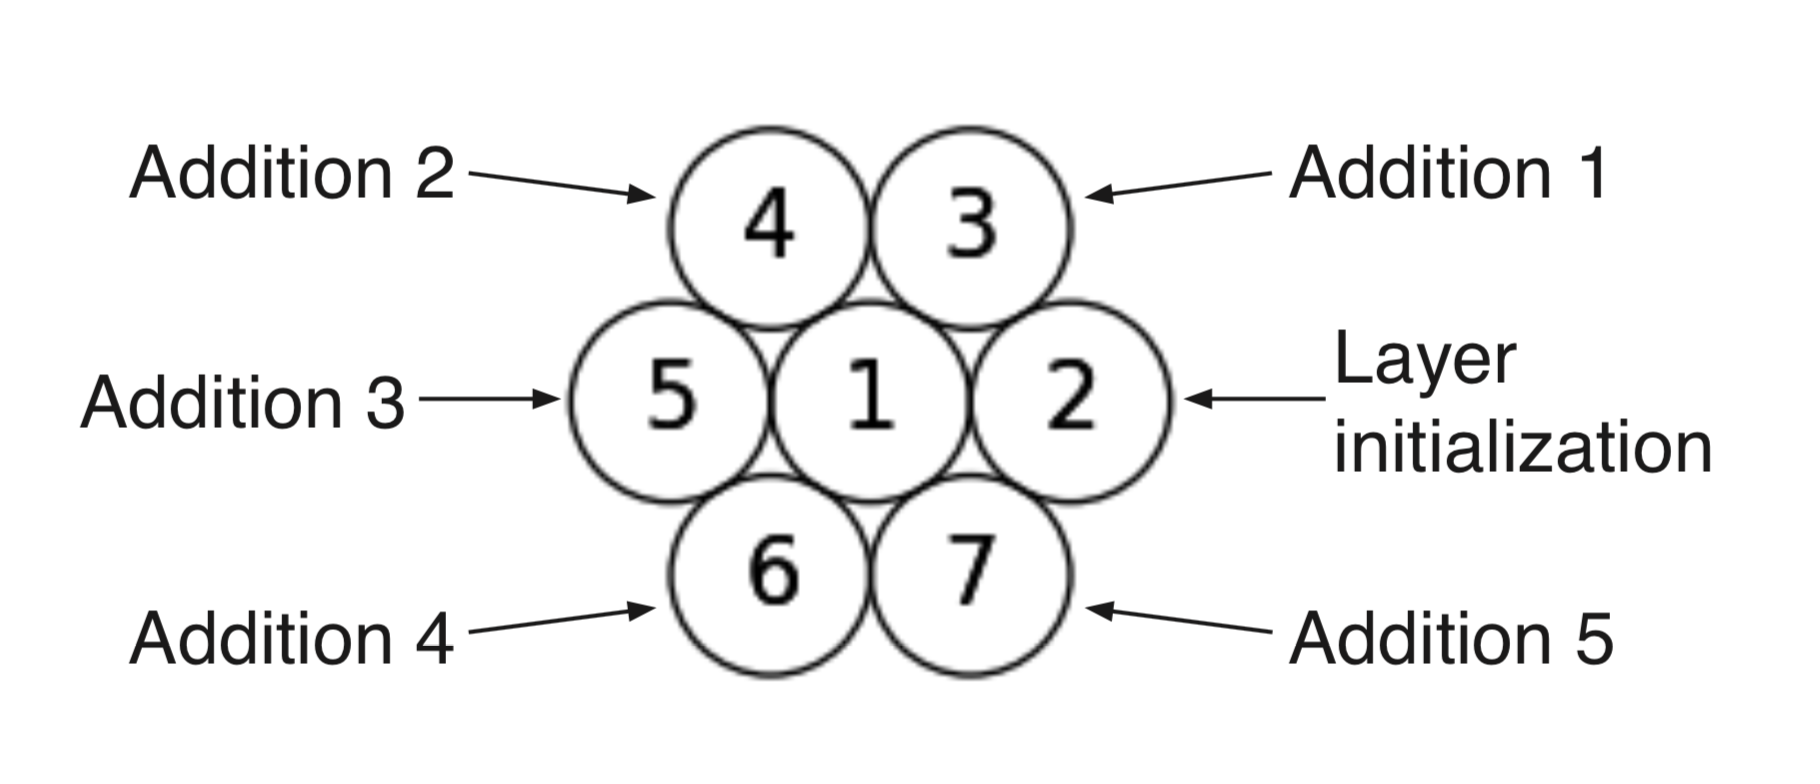
\includegraphics[width=\textwidth]{circles/layer_1}
	\caption{First actuator's layer.}
	\label{fig:appendix:sloan_structure:layer_1}
	\end{subfigure}
	
	\begin{subfigure}{0.70\textwidth}
	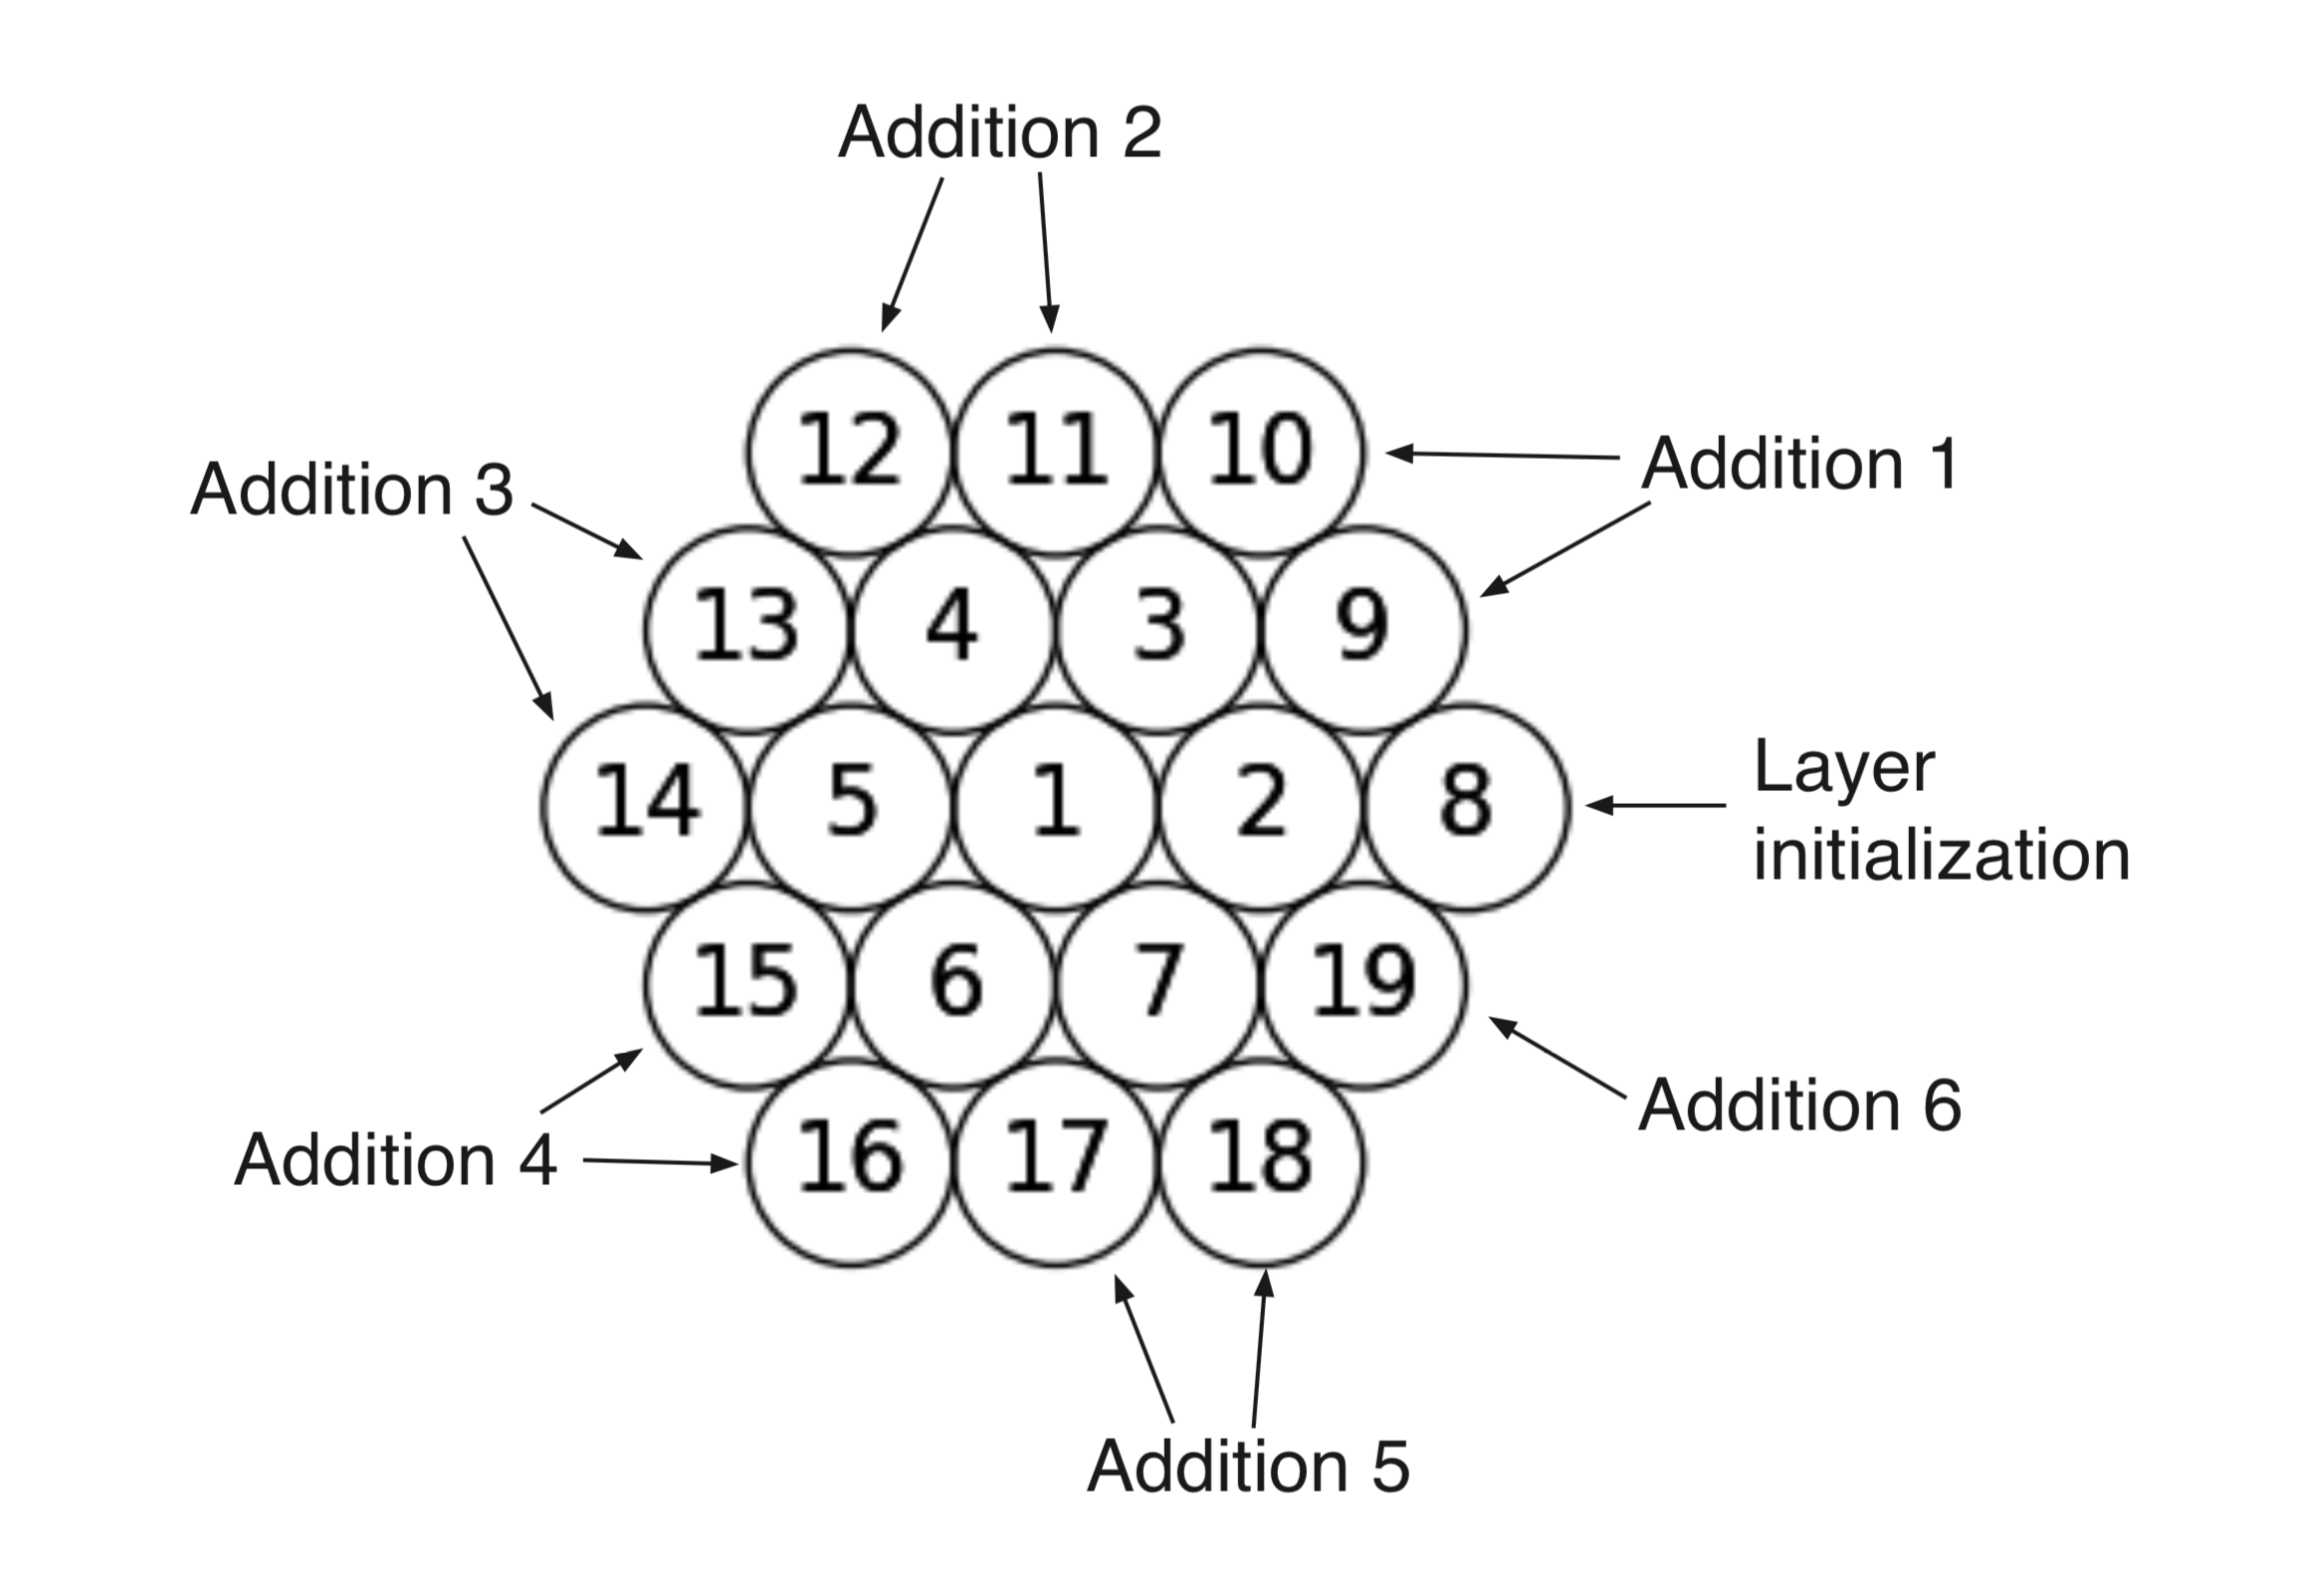
\includegraphics[width=\textwidth]{circles/layer_2}
	\caption{Second actuator's layer.}
	\label{fig:appendix:sloan_structure:layer_2}
	\end{subfigure}
	\caption{Actuators structure explanation: the initialisation creates an actuator at position (0, 0), layer initialisation then creates an actuator on the right, and each addition function creates an actuator close to the last actuator created. $i^{\textrm{th}}$ layer is built by initialising the layer, repeating addition functions 1-5 $i$ times, and finishing by repeating addition function 6 $(i-1)$ times.}
	\label{fig:appendix:sloan_structure}
\end{center}
\end{figure}


\begin{figure}[h]
\begin{center}
	\scriptsize{
	\begin{python}
position.append((0, 0))

def initialisation(num_circle):
    position.append((2*R*num_circle, 0))
    return

def addition_1():
    position.append(tuple((map(operator.add, position[(len(position)-1)], (-R, R * 3 ** 0.5)))))
    return

def addition_2():
    position.append(tuple((map(operator.add, position[(len(position)-1)], (-2*R, 0)))))
    return

def addition_3():
    position.append(tuple((map(operator.add, position[(len(position)-1)], (-R, -R * 3 ** 0.5)))))
    return

def addition_4():
    position.append(tuple((map(operator.add, position[(len(position)-1)], (R, - R * 3 ** 0.5)))))
    return

def addition_5():
    position.append(tuple((map(operator.add, position[(len(position)-1)], (2*R, 0)))))
    return

def addition_6():
    position.append(tuple((map(operator.add, position[(len(position)-1)], (R, R * 3 ** 0.5)))))
    return

def repeat_function(num_circle, function):
    for _ in range(num_circle):function()
    return

def layer_prod(layer):
    initialisation(layer)
    repeat_function(layer, addition_1)
    repeat_function(layer, addition_2)
    repeat_function(layer, addition_3)
    repeat_function(layer, addition_4)
    repeat_function(layer, addition_5)
    repeat_function((layer - 1), addition_6)
    return
	\end{python}
	}
	\caption{Code generating the hexagonal structure shown Figure \ref{fig:sloan:arrangement}. The first line creates the actuator at position (0, 0) (see Figure \ref{fig:appendix:sloan_structure:initialization}). Effects of functions initialisation and addition 1 to 6 are shown on Figure \ref{fig:appendix:sloan_structure:layer_1}. Upper layers (see Figure \ref{fig:appendix:sloan_structure:layer_2}) are built using functions repeat_function and layer_prod.}
	\label{fig:appendix:sloan_structure:code}
\end{center}
\end{figure}

